\section{Eletrônica}

\subsection{Necessidade de medição do nível de carga da bateria}

Um aspecto vital para o correto funcionamento do sistema, é a estimação da nível de carga da bateria, para que não haja danos na bateria por completa descarga ou que o sistema seja completamente desligado, não possibilitando sua comunicação com a central, em virtude de uma demanda de uso com carga insuficiente.

\subsection{Interface para o medidor de tensão da bateria}

A carga da bateria possui uma relação direta com a sua tensão, na qual será utilizada para leitura analógica pelo microcontrolador. De acordo com o datasheet da bateria utilizada, em 20\% da sua carga, sendo arbitrada como carga mínima para o sistema funcionar normalmente, a mesma apresenta 12V de tensão, enquanto na sua carga máxima, é apresentado 13V.
Tendo isto em vista, notou-se como necessário reduzir a escala deste nível de tensão máximo para 5V para que possa ser lido pela conversão AD do microcontrolador. Porém, quando esta redução é feita por um simples divisor de tensão resistivo, além de ser uma solução altamente ineficiente por drenar corrente o tempo inteiro, também gera uma saída que não aproveita muito bem a resolução de leitura do conversor AD.
A solução utilizada para medir a tensão da bateria de forma eficiente foi baseada em amplificador subtrator com referência fixa de tensão para modificar o offset da tensão da bateria reduzida, e também no uso de um MOSFET de uso geral para chavear todo o circuito de medição e liga-lo somente quando for requisitada a leitura da carga da bateria.

\begin{figure}[h]
	\centering
	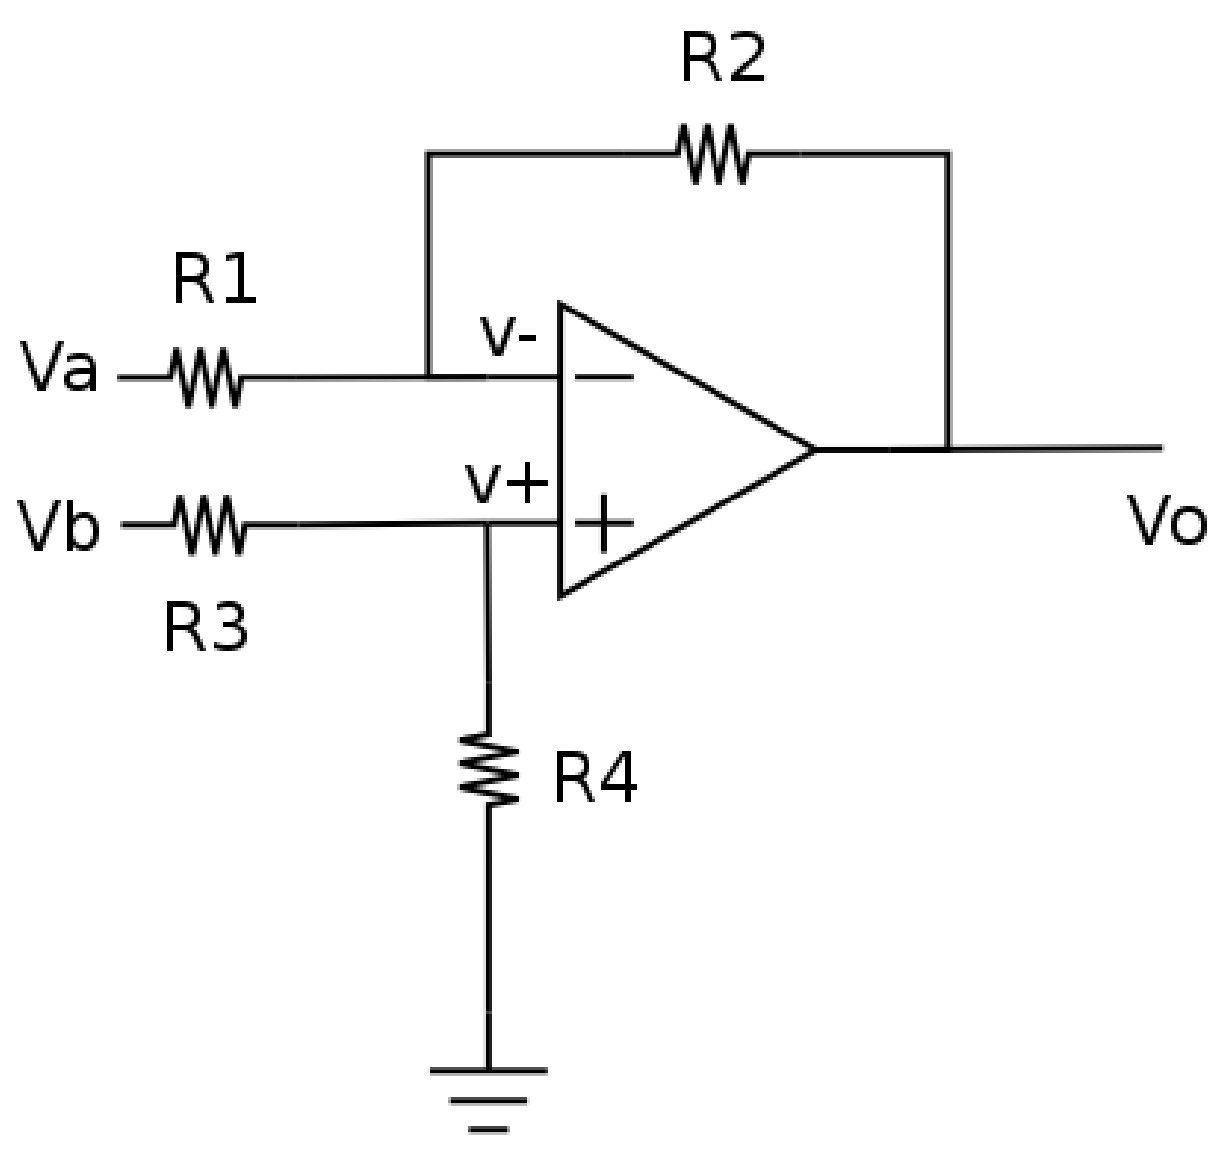
\includegraphics[keepaspectratio=true,scale=0.35]{figuras/amplif_sub_topo}
	\caption{ O circuito base para o amplificador subtrator.}
	\label{amplif_sub}
\end{figure}

\pagebreak

A relação entre a saída e as entradas desta topologia de amplificador são dadas pela equação	:
\begin{equation}
\label{div1}
V_{o}=V_{b}\frac{R_{4}(R_{1}+R{2})}{R_{1}(R_{3}+R{4})}-V_{a}\frac{R_{2}}{R_{1}}
\end{equation}

Em que na entrada Va é utilizada uma tensão fixa de aproximadamente 5V, na entrada Vb é ligada a tensão da bateria. A saída teórica prevista será um mapeamento de 13V a 12V para 5V a 0V. Com isto, monta-se o seguinte sistema:
$a13-b5 = 5$
$a12-b5 = 0$

A partir do mesmo, se encontram os dois primeiros valores dos resistores que são:
$b = R2/R1 = 1.2k/100$

Então, a partir destes resistores determinados, acha-se a relação entre os outros valores de resistências:
\begin{equation}
\label{div2}
a=\frac{R_{4}(R_{1}+R{2})}{R_{1}(R_{3}+R{4})}=\frac{R_{4}(13)}{R_{3}+R_{4}}
\end{equation}
$R3 = R4 8/5$

Sendo arbitrados os valores:

$R4 = 500, R3 = 800$

Porém, como na prática, nem todos os valores de resistores não são comerciais, a tensão de referência é levemente desviada e existirá uma zona morta de tensão referente a saturação negativa do AmpOp, será utilizado também um trimpot para calibrar a máxima tensão e o nível mínimo será dado pela tensão de saturação negativa do AmpOp, que na prática, é apresentada como resultado dos 12V da bateria.
A partir destas considerações feitas, projeta-se o circuito mostrado na figura \ref{bateria}

\begin{figure}[h]
	\centering
	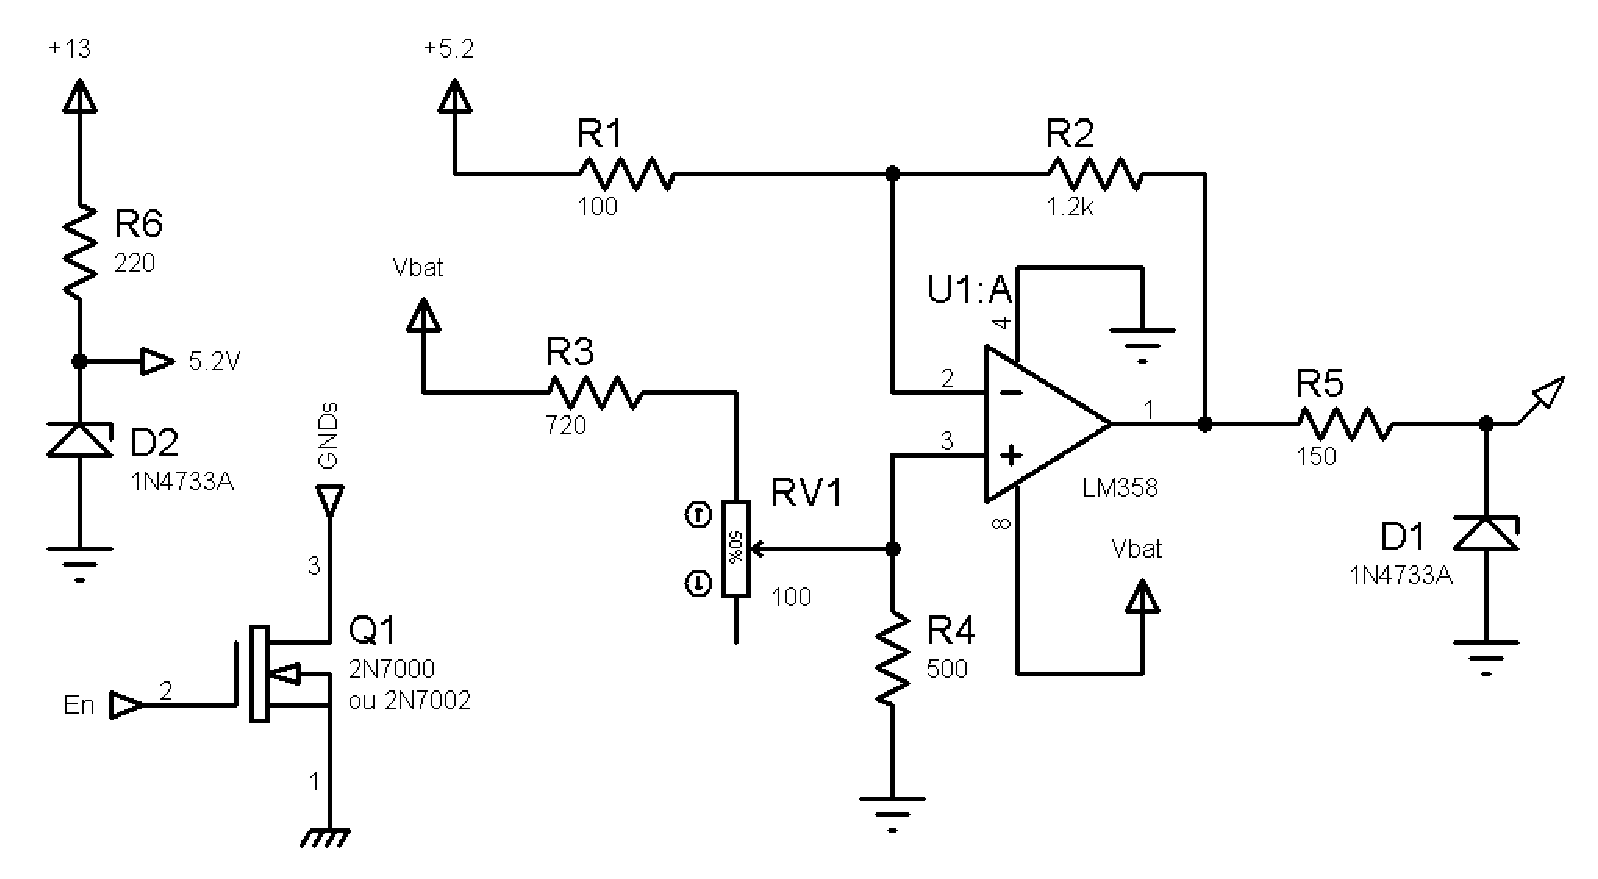
\includegraphics[keepaspectratio=true,scale=0.35]{figuras/bateria}
	\caption{ Circuito completo utilizado na medição de carga da bateria.}
	\label{bateria}
\end{figure}


\subsection{Sensor de pH}

Para a medição do pH foi usada a sonda e o módulo de instrumentação para amplificação do sinal apresentados na figura \ref{sonda_pH}.

\begin{figure}[h]
	\centering
	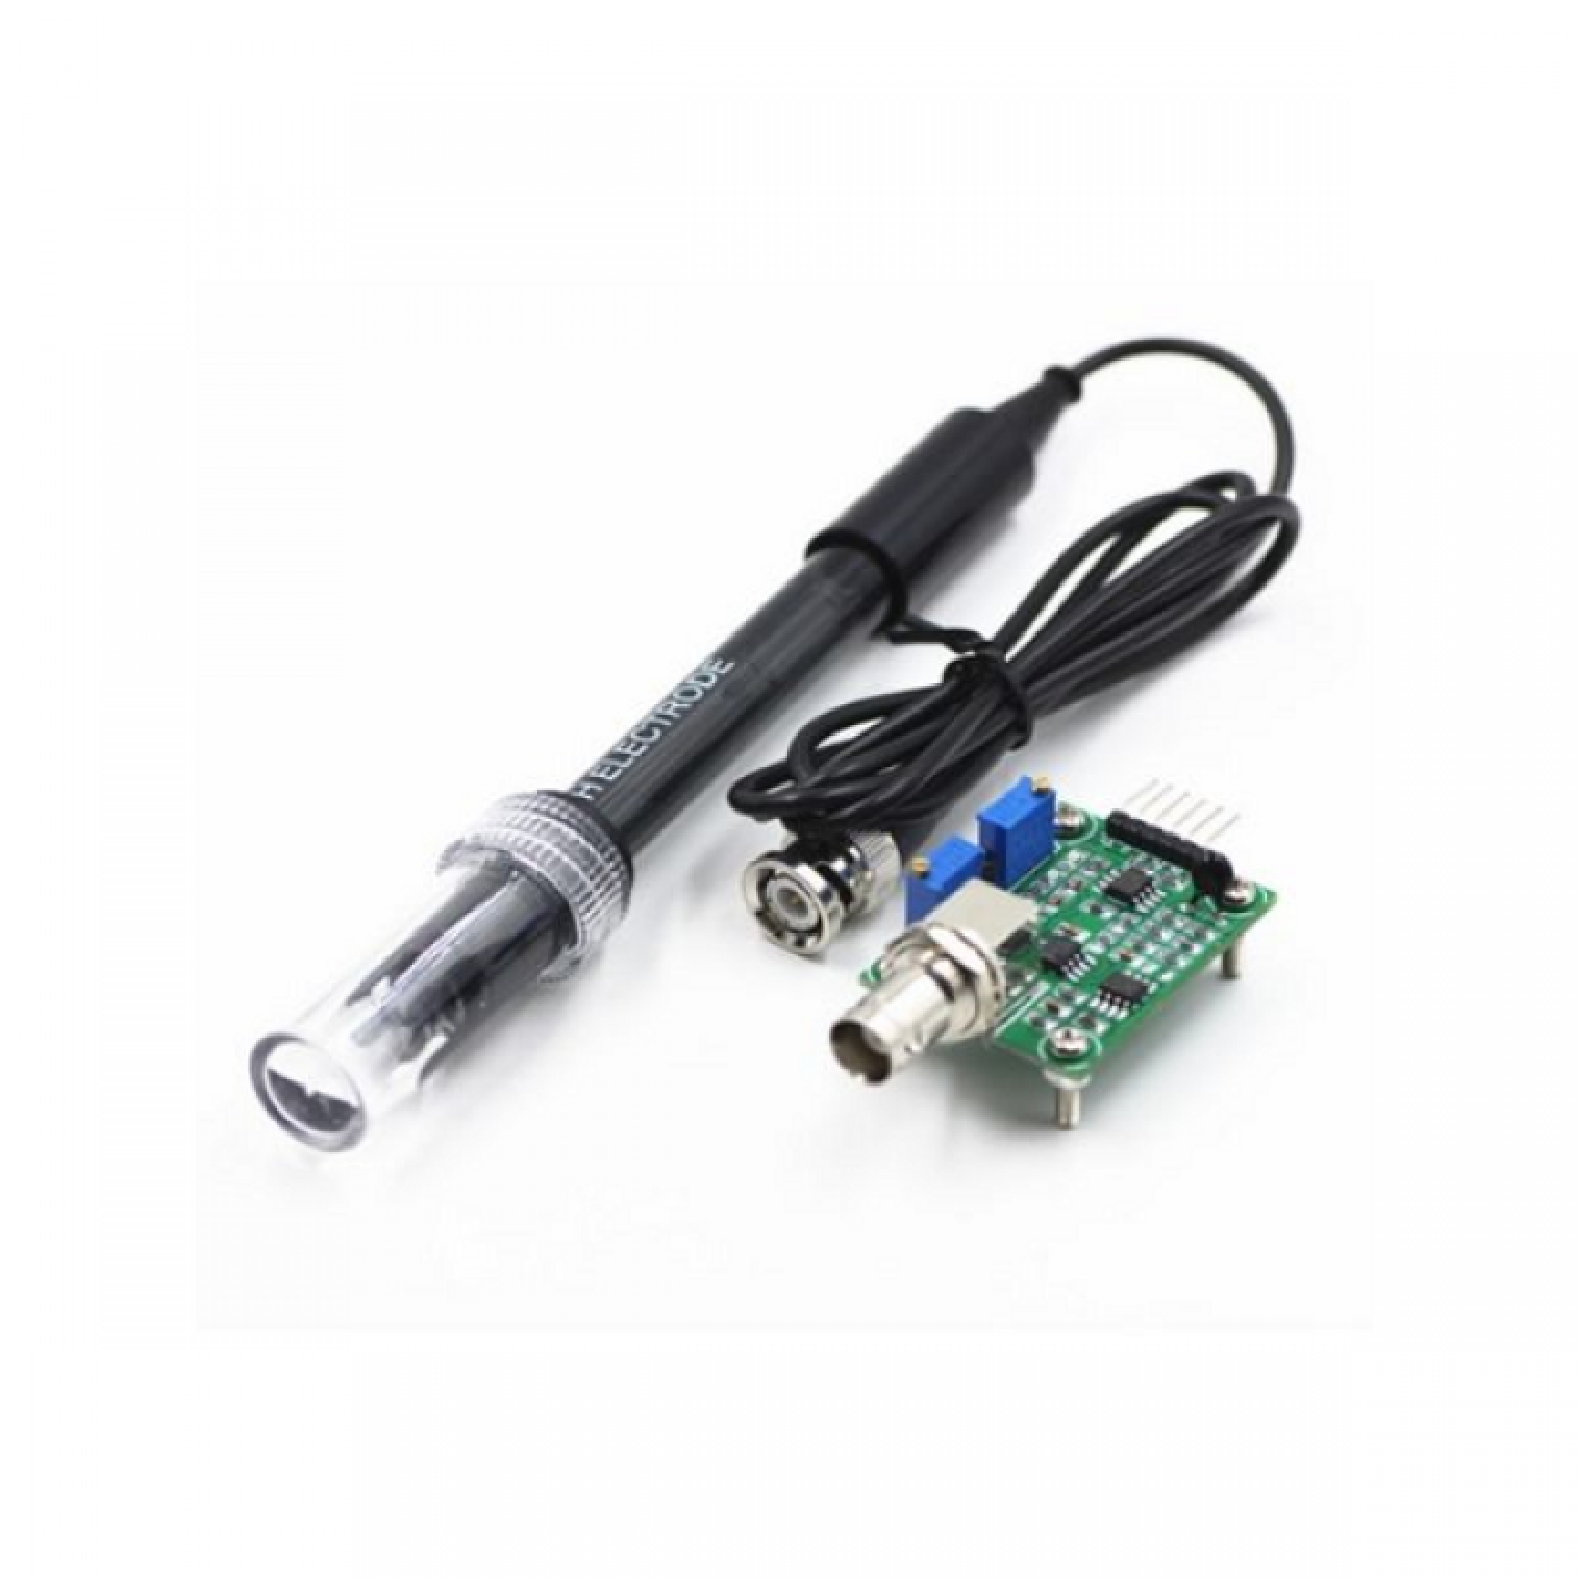
\includegraphics[keepaspectratio=true,scale=0.35]{figuras/sonda_pH}
	\caption{Sonda e módulo utilizados para a medição do pH.}
	\label{sonda_pH}
\end{figure}

A figura \ref{pH_curve} ilustra a curva fornecida pelo fabricante por esta sonda em suas medições de volumes de uma solução de soda cáustica dissolvida em água. Essa curva fornecida pela sonda assume padrão próximo ao linear entre valores 4 e 9.

\begin{figure}[h]
	\centering
	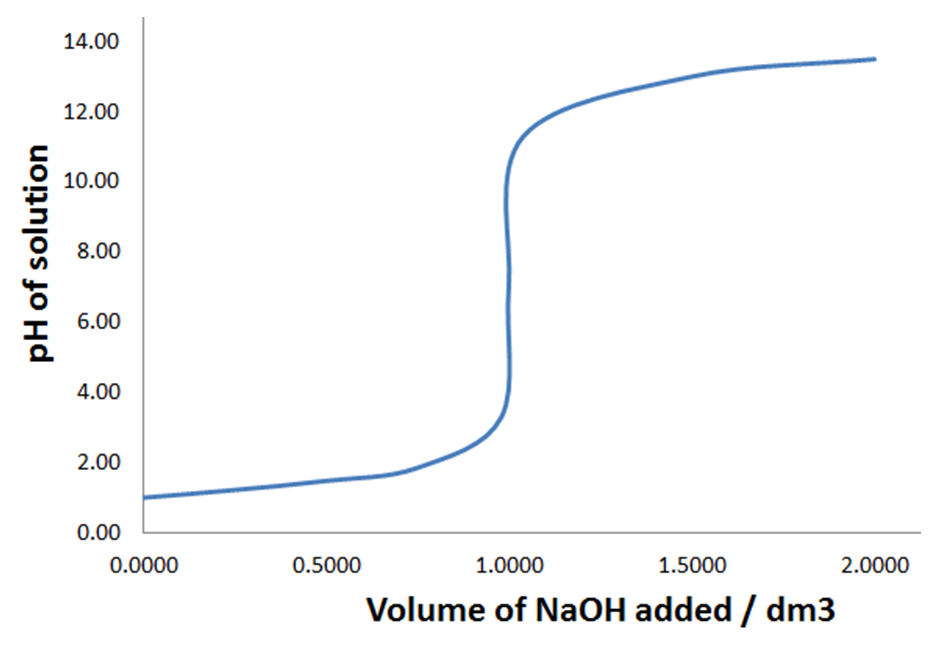
\includegraphics[keepaspectratio=true,scale=0.7]{figuras/pH_curve}
	\caption{Curva de pH.}
	\label{pH_curve}
\end{figure}

\pagebreak

A sonda foi calibrada no laboratório de química da FGA - UnB com auxílio técnico. Por padrão, para a calibração, são usadas duas amostras: uma de pH 4 e outra de pH 7. A curva obtida através da calibração realizada é apresentada na figura \ref{pH_cal}

\begin{figure}[h]
	\centering
	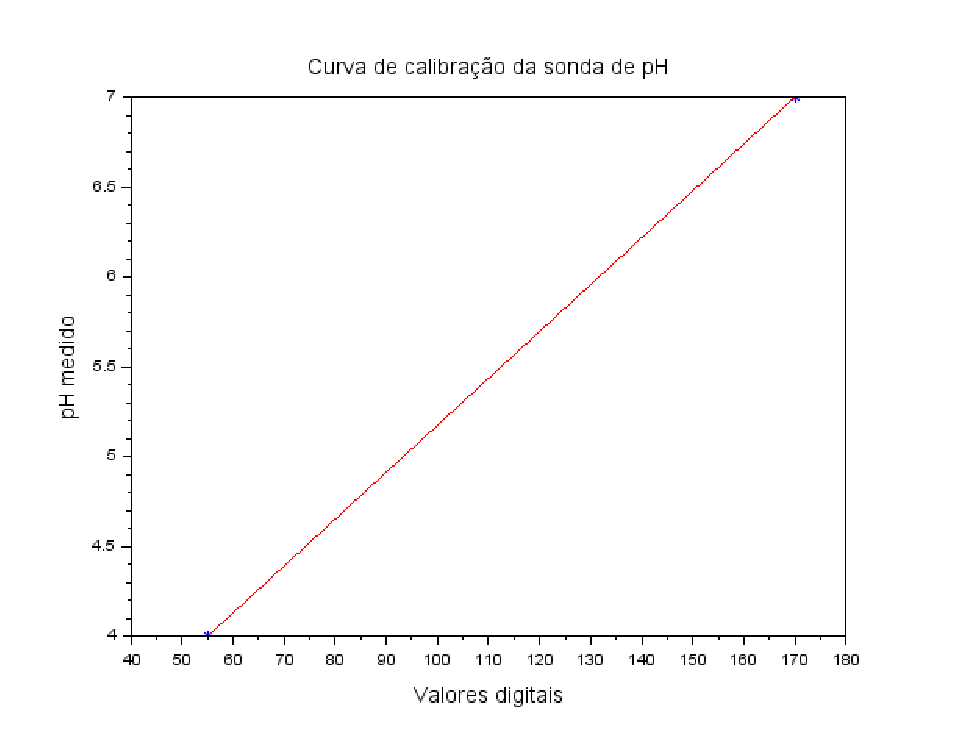
\includegraphics[keepaspectratio=true,scale=0.7]{figuras/pH_cal}
	\caption{Curva de calibração da sonda de pH.}
	\label{pH_cal}
\end{figure}

A função obtida para a calibração é mostrada na equação \ref{ph1}.

\begin{equation}
\label{ph1}
    pH = 0.026087x + 2.565
\end{equation}

Sendo:

$pH$ = valor de pH;

$x$ = valor fornecido pelo ADC.

\subsection{Sistema de Controle Para a Alimentação}

Para o controle da quantidade de ração despejada foi necessário projetar um sistema de controle embarcado que faz parte da placa presente nos tanques. Um sistema de controle é um conjunto de dispositivos que trabalham para alterarem o comportamento de um sistema, a seguinte figura ilustra os blocos que compõem um sistema de controle:

\begin{figure}[h]
\centering
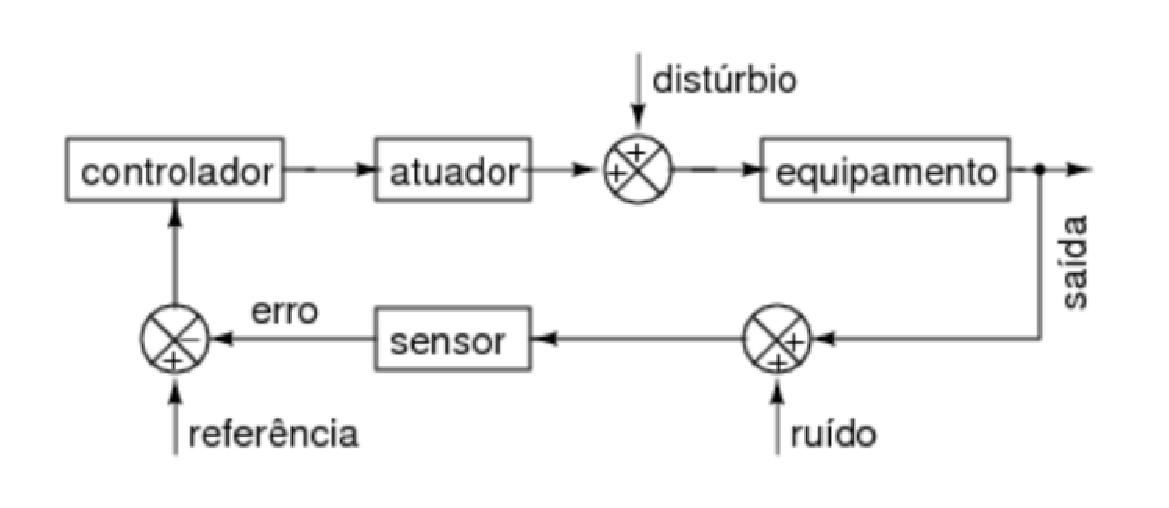
\includegraphics[keepaspectratio=true,scale=0.6]{figuras/sistema_de_controle}
\caption{Diagrama de Blocos de um Sistema de Controle.}
\label{blocoscontrole}
\end{figure}

O sensor é o dispositivo que converte a grandeza física a ser monitorada, no caso do projeto o peso da ração, em um sinal elétrico. Este sinal elétrico é enviado ao microcontrolador para que ele seja comparado com o sinal de referência, que no caso é o peso da ração que deseja-se despejar, caso o valor de ração que se encontra no recipiente dosador ainda esteja abaixo do desejado o sistema continuará a acionar o atuador, que no caso do projeto é o motor CC que controla o fuso que despeja a ração. O fuso continuará despejando ração no recipiente dosador até que o valor desejado seja atingido, quando o sensor medir um valor que ultrapasse o valor desejado o microcontrolador irá verificar e parar o motor do fuso e acionar o motor de passo que abre a comporta do dosador, despejando a ração. Abaixo cada componente deste sistema é explicado mais detalhadamente.

Antes do sistema de alimentação iniciar é necessário verificar se está no horário para a alimentação, caso esteja o procedimento para a alimentação é chamado e o valor da quantidade de ração é passado para a função como mostra o seguinte trecho de código:

\begin{figure}[!h]
\centering 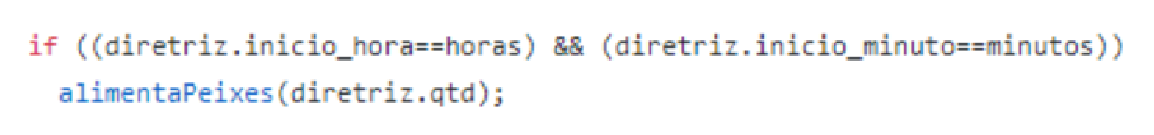
\includegraphics[scale=0.5]{figuras/codigo_controle}
\label{codigo_controle1}
 \end{figure}

O seguinte trecho de código mostra como é implementada a comparação entre a variável medida (peso atual de ração no recipiente) e o valor desejado:

\begin{figure}[!h]
\centering 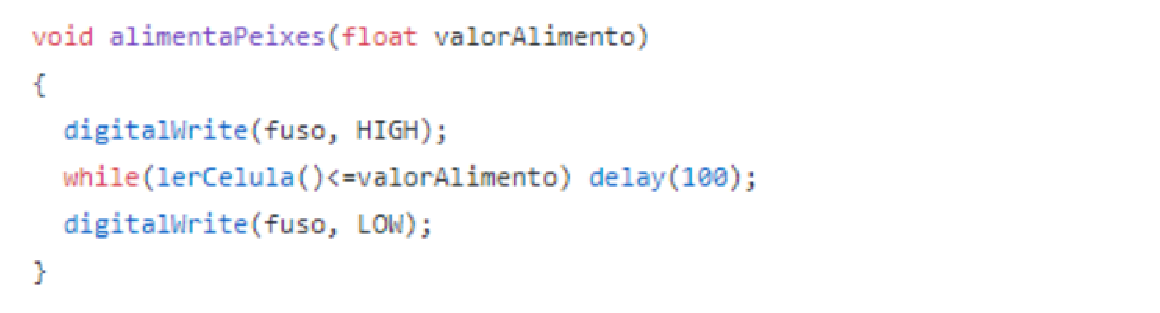
\includegraphics[scale=0.6]{figuras/controle2_codigo}
\label{codigo_controle2}
 \end{figure}

O pino que envia o sinal para que o motor do fuso que retira a ração do reservatório e a deposita no dosador é colocado em nível alto, começa-se então o processo de comparação  em um laço while. A função lerCelula() que será explicada mais a frente faz a aquisição dos valores lidos pela célula de carga e realiza a calibração, este valor é comparado com o desejado, quando o ultrapassar o motor é então desligado.

Para a medição do peso de ração recebida pelo dosador escolheu-se utilizar células de carga e um circuito HX711 condicionador de sinais para enviar as medidas para o ATmega. Uma célula de carga é um transdutor que converte uma força feita sobre ele, no caso do projeto, uma carga exercida pela ração, em um sinal elétrico. Este sinal pode ser uma mudança de corrente, uma mudança de tensão ou de frequência dependendo da célula e do circuito em que ela está implementada. As células de carga podem ser de dois tipos: resistiva, que mudam sua resistência quando uma força é aplicada sobre ela, e as capacitivas, que alteram sua capacitância ao ter uma força aplicada sobre ela \cite{loadcell}. A célula de carga utilizada foi do tipo resistiva, ela possui um strain gauge acoplado em sua superfície para medir as variações de compressão.

Um \textit{strain gauge} é um resistor que tem sua resistência variando de acordo com a quantidade de deformação a qual ele é submetido, ele é um dos resistores mais usados para medir peso.  Um strain gauge pode ser visto na figura abaixo:


\begin{figure}[!h]
\centering 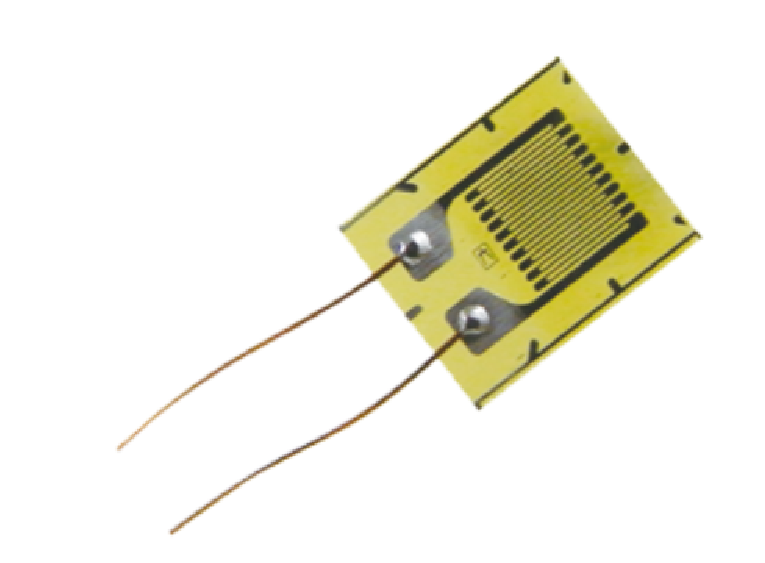
\includegraphics[scale=0.5]{figuras/strain_gage}
\caption{Strain Gauge}
\label{straingauge}
 \end{figure}

A figura abaixo apresenta a célula de carga utilizada, ela suporta até 5kg, mas o peso a ser suportado por ela é de, no máximo 10kg, por este motivo foram usadas duas células conectadas em paralelo. O strain gauge presente na superfície da célula de carga forma, em conjunto com três resistores fixos de aproximadamente 1K, uma ponte de Wheatstone para fazer as medições na peso.

\begin{figure}[!h]
\centering 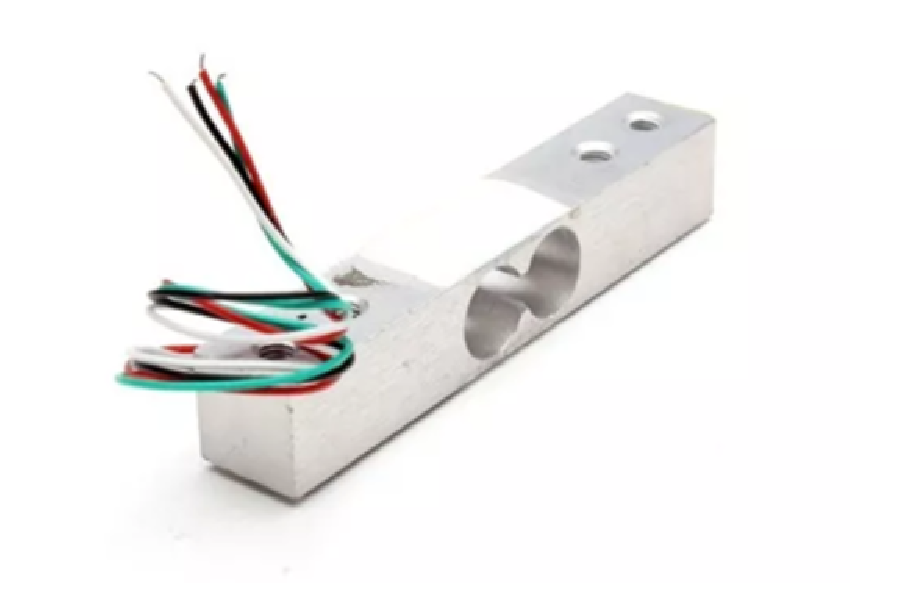
\includegraphics[scale=0.5]{figuras/celula_de_carga}
\caption{Célula de carga de 5kg utilizada no projeto.}
\label{celulacarga}
 \end{figure}

A ponte de Wheatstone é usada para traduzir a deformação em uma tensão. Um diagrama de uma ponte de Wheatstone é mostrado na figura abaixo:

\begin{figure}[!h]
\centering 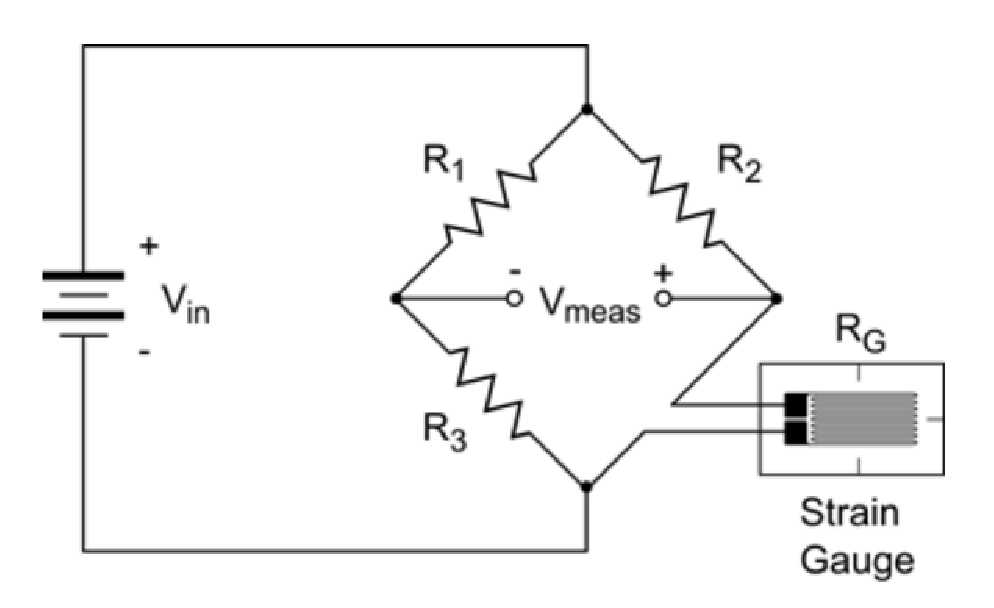
\includegraphics[scale=0.6]{figuras/ponte_de_wheatstone}
\caption{ Ponte de Wheatstone encontrada na célula de carga}
\label{wheatstone}
 \end{figure}

A equação \ref{cont4} fornece o valor da tensão $V_{meas}$ em função da deformação do strain gauge, considerando que $R_{1}=R_{2}=R_{3}=R$ e $R_{G}=R+\Delta R$.

\begin{equation}
\label{cont4}
V_{meas}=V_{in} \frac{-\Delta R}{4R+2\Delta R} \approx V_{meas}=V_{in} \frac{-\Delta R}{4R}
\end{equation}

É importante lembrar que o valor de $R=500\Omega$ já que duas pontes estão em paralelo devido ao uso de duas células de carga.

A variação de tensão gerada pela ponte de Wheatstone em resposta à carga colocada sobre as células de carga ainda é baixa e precisa ser amplificada, além disto é necessário que  sinal seja convertido em digital, para isto foi usado o módulo HX711 de 24 bits. Uma ilustração que apresenta um diagrama dos blocos que constituem o módulo é apresentado na figura abaixo:

\begin{figure}[!h]
\centering 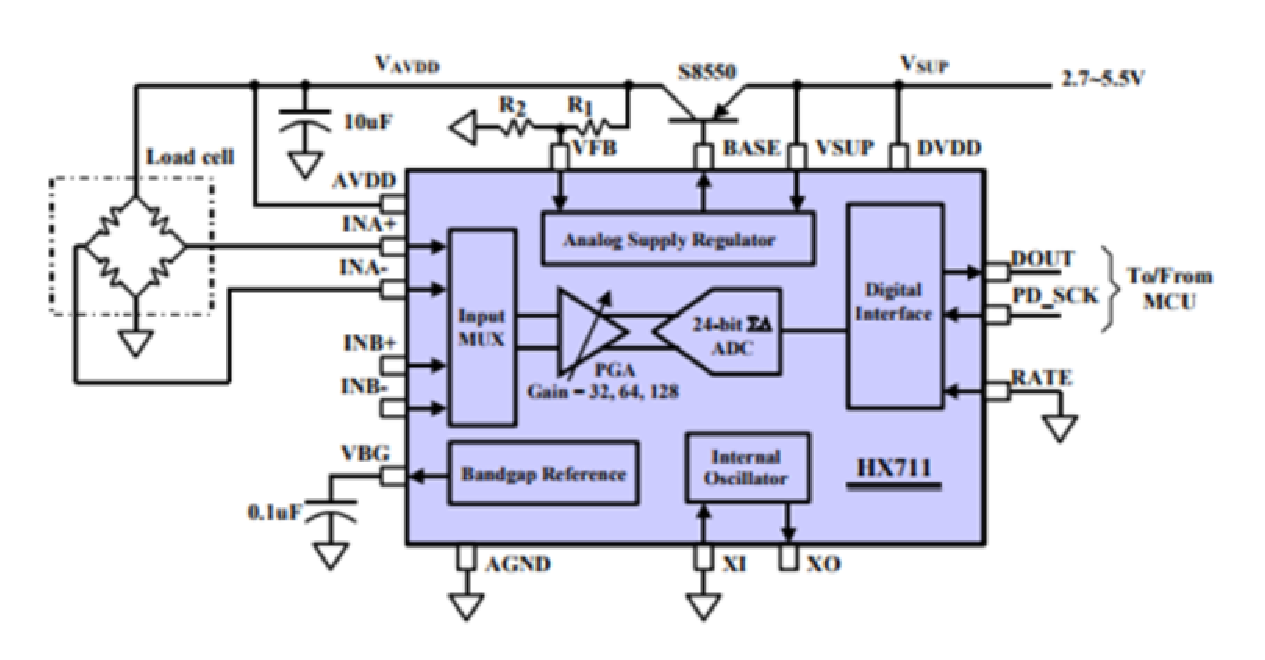
\includegraphics[scale=0.7]{figuras/hx711}
\caption{Diagrama de blocos para do módulo Hx711.}
\label{hx711}
 \end{figure}

\pagebreak

Ele possui dois canais A e B de entrada para o sinal diferencial que no caso do projeto é o sinal que sai da ponte de Wheatstone, estes canais podem ser selecionados pelo multiplexador interno. Este sinal é amplificado pelo PGA (\textit{Programmable Gain Amplifier}) que pode dar ganho de 64 e 128 para o canal A e 32 para o canal B, o sinal de saída do PGA passa por um conversor AD antes de ser armazenados em seus registradores. Os dados são recuperados dos registradores através dos pinos DOUT e PD\_SCK, o pino DOUT permanece em nível alto até o momento em que a conversão está pronta e os dados podem ser recuperados, neste momento o nível do pino DOUT vai pra baixo. Aplicando 25 pulsos em PD\_SCK os próximos dados obtidos serão do canal A com ganho de 128, 26 pulsos os próximos dados obtidos serão do canal B com ganho de 32 e 27 pulsos os próximos dados obtidos serão do canal A com ganho de 64 \cite{avia:hx711}.

A seguinte função realiza o trabalho de fazer a leitura do módulo, ela é baseada no código fornecido pelo datasheet do circuito e sempre pega o valor que vem do canal A com ganho de 128:

\begin{figure}[!h]
\centering 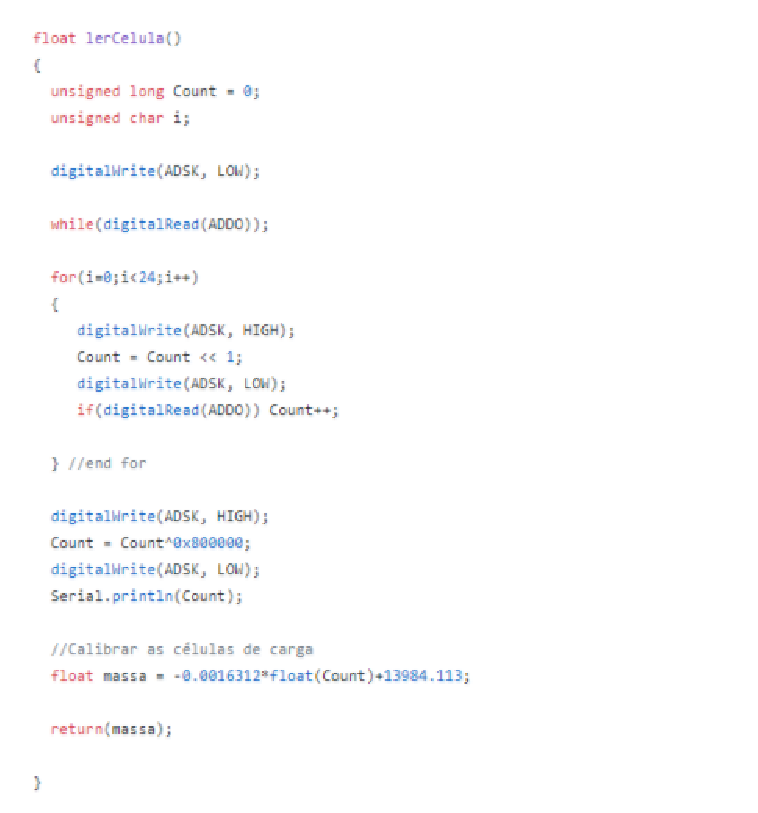
\includegraphics[scale=0.9]{figuras/hx711_codigo}

\label{hx711codigo}
\end{figure}

\pagebreak

A função também converte o valor digital de 24 bits vindo do CI para o valor equivalente em massa, para isto foi necessário realizar a calibração das células. O processo de calibração estática consiste em alterar apenas uma variável de entrada e verificar como a saída se comporta com aquela alteração, após o comportamento ser verificado uma função de ajuste que relaciona os valores de saída com os de entrada é traçada. A resultado obtido é apresentado no gráfico abaixo:

\begin{figure}[!h]
\centering 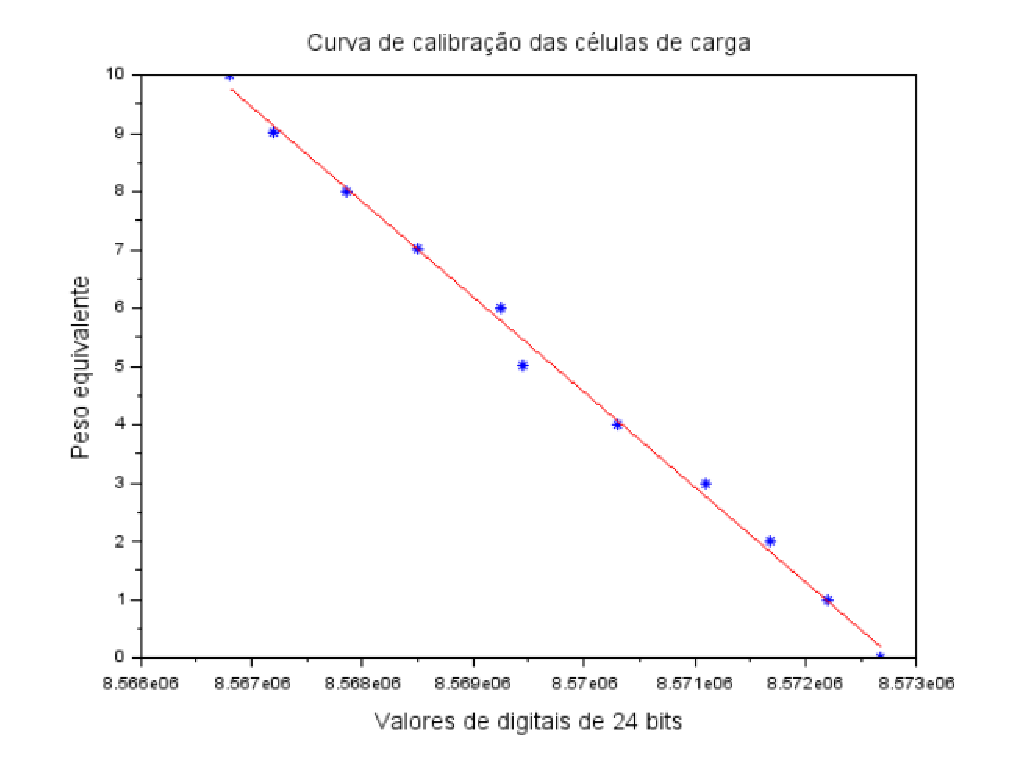
\includegraphics[scale=0.7]{figuras/calibracao_celula_de_carga}
\label{calibracaocelula}
\end{figure}

\pagebreak

\subsection{Filtro para leitura da célula de carga}

O sistema de medição de peso do dosador por célula de carga, apesar de ser funcional, apresenta dois problemas a serem contornados: O primeiro inconveniente é o alto nível de ruído inerente da leitura de tensão das células de carga. Já o segundo é, em virtude do sistema estar flutuando encima da água, está vulnerável a todas as ondulações da água e oscilações da estrutura.
Tendo isto em vista, foi concebido um filtro digital para as entradas lidas da interface da célula de carga. Os ruídos são vistos como um sinal aleatório de offset zero e as oscilações são modeladas como um sinal senoidal de alta amplitude e baixa frequência, considerando algo maior que 0,2 Hz. O sinal do peso obtido é previsto como uma rampa crescente que funciona de forma semelhante a um nível DC.
A partir destas considerações, foi concebido um filtro FIR passa-baixas, com frequência de corte de 0,2 Hz. Foi levado em consideração que quanto menor for a frequência de corte, mais demorada será a resposta do sistema, e quanto menor for a banda de transição e os ripples, mais elementos de memórias e operações aritméticas serão necessários.
Para o projeto deste filtro, foi utilizada a ferramenta online Tfilter \cite{tfilter}. Ela apresenta como vantagem uma interface bem visual e bastante intuitiva, além de mostrar os resultados previstos em tempo real. Após diversos testes, o filtro obtido possui uma banda de rejeição de 0,1 Hz a 0,2 Hz, ripple da banda de passagem de 4.2 dB, nível de rejeição de -40 dB e 127 elementos de memória (taps).
Foi desenvolvido um script de Matlab® para testes e obtenção de outros valores importantes. Primeiro foram armazenados os coeficiente obtidos do Tfilter em no array h em precisão float. Em seguida, os coeficientes foram convertidos em inteiros de 8 bits e maximizados para implementação no microcontrolador. Em virtude disto, o filtro deixa de ter ganho unitário, que é facilmente normalizado utilizando-se um divisor comum proveniente da soma de todos os coeficientes. O algoritmo que realiza tudo isto está expresso na figura \ref{rfreq}:

\begin{figure}[h]
	\centering
	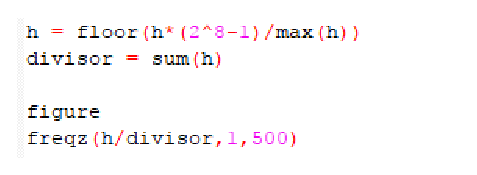
\includegraphics[keepaspectratio=true,scale=0.9]{figuras/rfreq}
	\caption{}
	\label{rfreq}
\end{figure}

\begin{figure}[h]
	\centering
	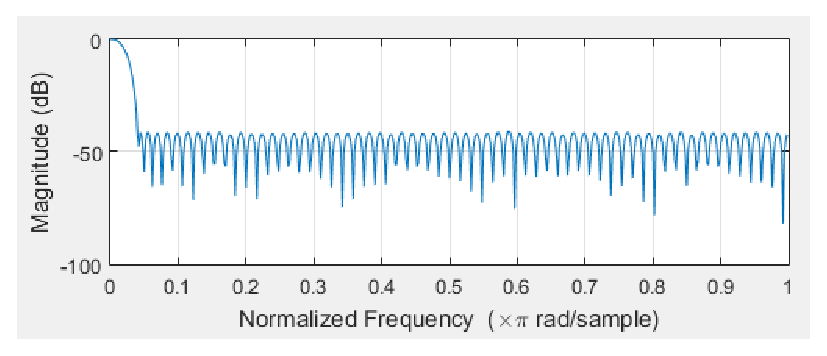
\includegraphics[keepaspectratio=true,scale=0.9]{figuras/freqz}
	\caption{Resposta em frequência obtida do filtro reduzido a ser implementado.}
	\label{freqz}
\end{figure}

Em seguida é realizado testes da resposta do filtro. O algoritmo expresso na figura \ref{convolu} implementa uma convolução do filtro com uma entrada x arbitrária, que para emular o sistema, é utilizada uma rampa.

\begin{figure}[h]
	\centering
	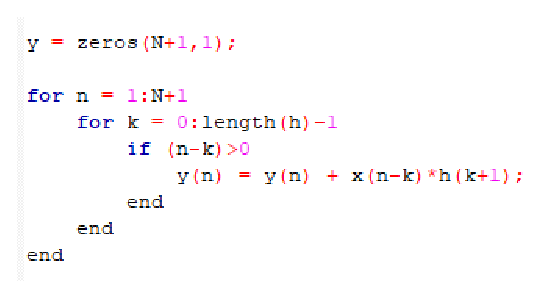
\includegraphics[keepaspectratio=true,scale=0.9]{figuras/convolu}
	\caption{}
	\label{convolu}
\end{figure}

No primeiro teste também é introduzido um alto nível de ruído junto com a rampa, cujo resultado está expresso na figura /ref{ruido}.

\begin{figure}[h]
	\centering
	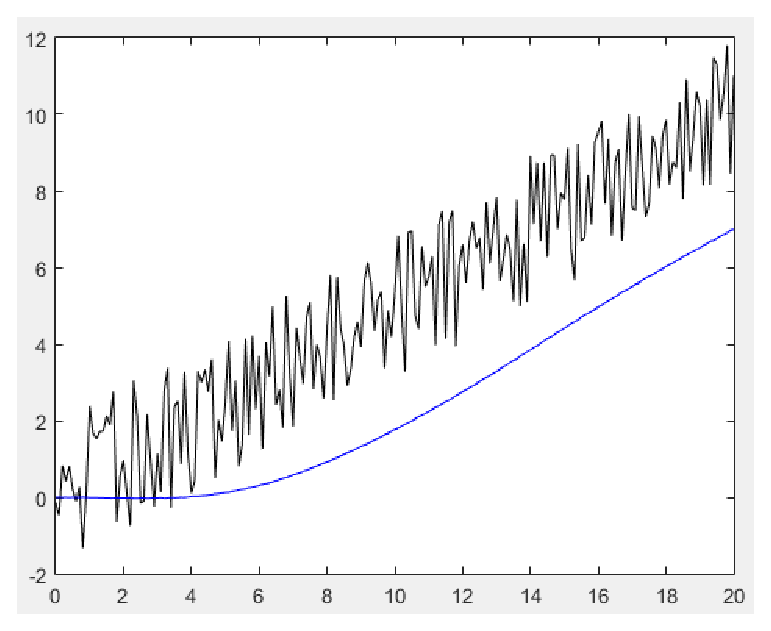
\includegraphics[keepaspectratio=true,scale=0.7]{figuras/ruido}
	\caption{}
	\label{ruido}
\end{figure}

Observa-se que a saída resultante encontra-se bastante limpa e com um atraso de aproximadamente 7s. Este atraso pode ser contornado prevendo-se o erro através do fluxo médio medido. No segundo teste é adicionado um sinal senoidal de 0,2 Hz e algum ruído junto com a rampa, que emulam o comportamento esperado durante 1 minuto de despejo, cujo resultado está expresso na figura \ref{osc}.

\begin{figure}[h]
	\centering
	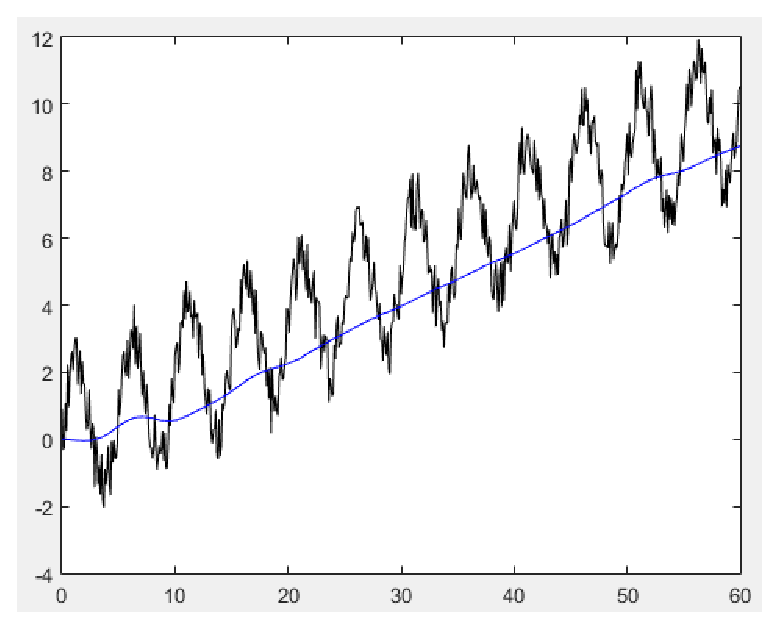
\includegraphics[keepaspectratio=true,scale=0.7]{figuras/osc}
	\caption{}
	\label{osc}
\end{figure}

Observa-se que as oscilações são bastante atenuadas e a resposta acompanha a subida do sinal de forma estável.

\subsection{Implementação do filtro de leitura do peso para o ATmega}

Para implementação no microcontrolador, são feitas as definições dos coeficientes do filtro, divisor de normalização, ordem do filtro e elementos de memória.

\begin{figure}[h]
	\centering
	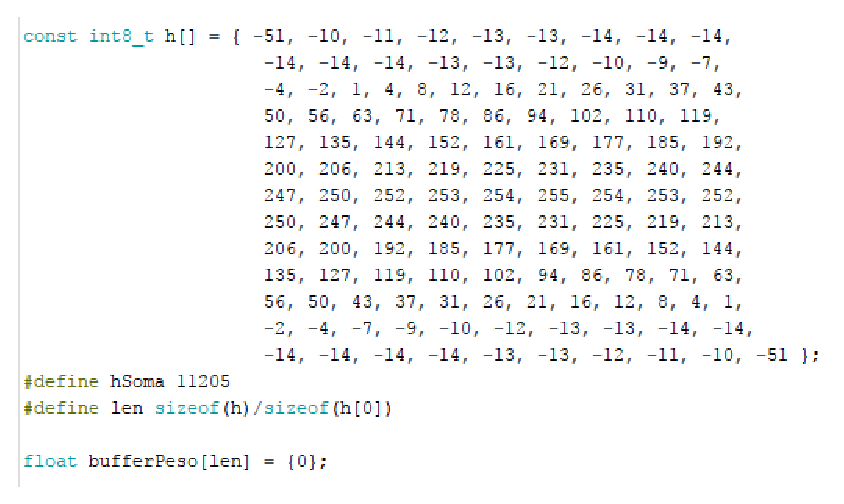
\includegraphics[keepaspectratio=true,scale=0.7]{figuras/alg0}
	\caption{ Definições em sintaxe C++ com alguns valores obtidos do Matlab.}
	\label{alg0}
\end{figure}

Em seguida é implementada a função de filtragem de um sinal dado que recebe os elementos de memória e retorna como saída o valor já normalizado.

\begin{figure}[h]
	\centering
	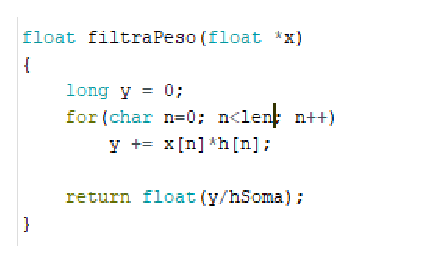
\includegraphics[keepaspectratio=true,scale=0.7]{figuras/alg1}
	\caption{ Implementação da convolução dos coeficientes do filtro com entradas passadas.}
	\label{alg1}
\end{figure}

Também é implementada uma função que realiza o deslocamento dos espaços de memória dos valores passados.

\begin{figure}[h]
	\centering
	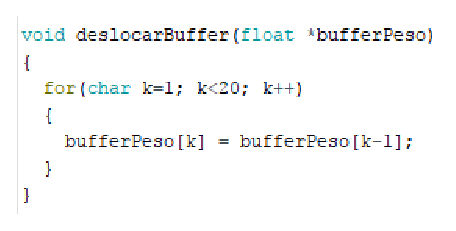
\includegraphics[keepaspectratio=true,scale=0.7]{figuras/alg2}
	\label{alg2}
\end{figure}

E por último, é implementada a função que recebe os valores brutos lidos das células de carga e entrega o valor filtrado

\begin{figure}[h]
	\centering
	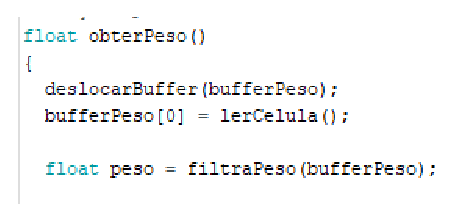
\includegraphics[keepaspectratio=true,scale=0.7]{figuras/alg3}
	\caption{ Implementação da convolução dos coeficientes do filtro com entradas passadas.}
	\label{alg3}
\end{figure}





A curva obtida foi colocada dentro da função lerCelula() para fazer a conversão.

Para ligar e desligar o motor do fuso escolheu-se utilizar o relé HJR1-2C que será acionado pelo transistor TBJ BC548. o relé suporta até 2A o que é suficiente já que a corrente do motor é de 1,58A.



\subsection{Sistema de Comunicação}

A comunicação entre os tanques e a base, bem como o sistema em geral são ilustrados pela figura \ref{diagramacomunicacao}

\begin{figure}[!h]
\centering 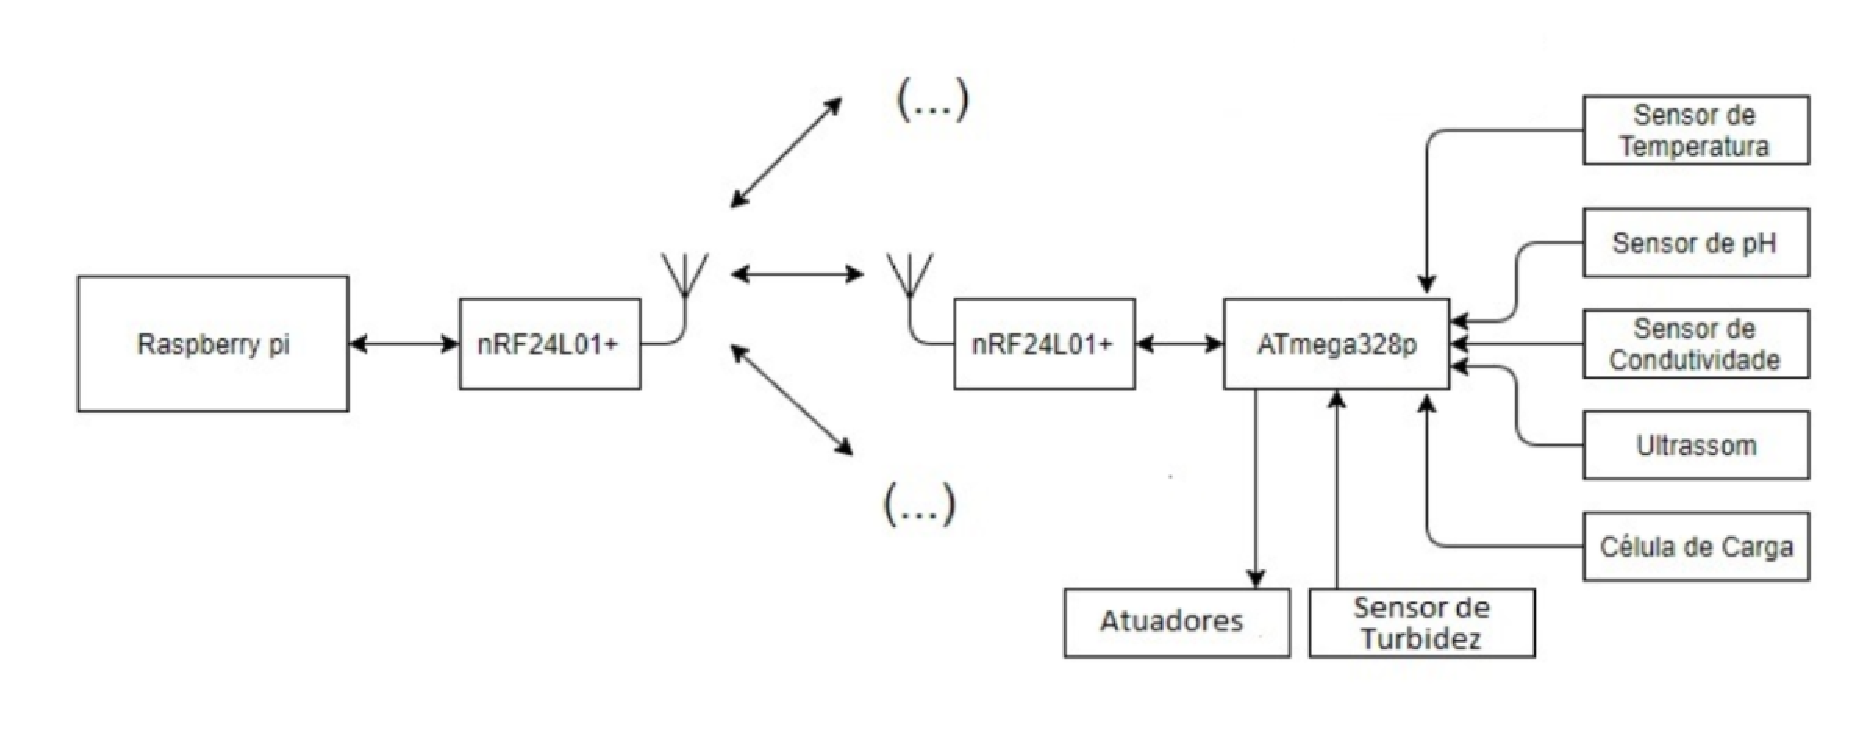
\includegraphics[scale=0.4]{figuras/diagrama_de_comunicacao}
\caption{Diagrama de Blocos do sistema.}
\label{diagramacomunicacao}
 \end{figure}

O módulo utilizado para a comunicação entre os dispositivos foi o módulo nRF24L01+. Este módulo contém um chip transceptor de 2,4 GHz para uso em aplicações \textit{wireless} de baixo consumo de potência, ele é configurado pelo microcontrolador ao qual ele está acoplado através de um protocolo \textit{Serial Peripheral Interface} (SPI). O transceptor pode ser  configurado através de registradores acessados por SPI.

Para assegurar a comunicação entre os dispositivos que fazem parte da rede foi necessário estimar a distância máxima que duas antenas que se comunicam podem ter entre elas. Levou-se em consideração a distância máxima entre a central e o tanque mais longe que é de 200m e que os tanques estão alinhados. Para fazer a estimativa teórica desta distância é necessário calcular as perdas e ganhos ao longo do caminho do sistema de transmissão, isto é feito com o cálculo denominado \textit{Link Budget}. Ele leva em consideração a potência de saída fornecida pelo transceptor, os ganhos das antenas, as perdas e ganhos a longo do caminho e a sensibilidade de recepção do transceptor. Este cálculo é também usado para verificar se os dispositivos escolhidos cumprem as exigências do projeto.  A equação \ref{com1} apresenta, em termos gerais, este cálculo.

\begin{equation}
\label{com1}
	P_{R} (dBm) = P_{T} (dBm) + ganhos (dB) - perdas (dB)
\end{equation}

Sendo $P_{R}$ a potência recebida e $P_{T}$ a potência transmitida \cite{ianpoole}.
Os seguintes pontos são levados em consideração para a realização do cálculo de distância máxima, sendo eles consequência das condições em que o sistema estará inserido:

\begin{itemize}
\item As antenas se encontram em um mesmo plano;
\item Não existem obstáculos entre elas pois estão localizadas em um plano aberto;
\item São usadas antenas omnidirecionais cujo ganho (em diretividade) máximo especificado é o ganho para todas as direções do plano perpendicular a elas.
\end{itemize}

Sabendo que os ganhos no percurso são os ganhos das antenas e a perda é a perda de caminho no espaço livre, e por não haverem obstáculos entre as duas antenas, pode-se utilizar então a equação \ref{com2}, denominada Equação de Friis, inicialmente proposta em \cite{1697062}, para estimar a distância máxima.

\begin{equation}
\label{com2}
\frac{P_{R}}{P_{T}} = G(\theta_{T},\phi_{T})G(\theta_{T},\phi_{T})\left ( \frac{\lambda _{0}}{4 \pi d} \right )^{2}
\end{equation}

Onde:

$P_{R}$ = potência recebida medida em Watts [W];

$P_{T}$ = potência transmitida medida em Watts [W];

$G(\theta_{T},\phi_{T})$ = ganho em diretividade da antena transmissora;

$G(\theta_{T},\phi_{T})$ = ganho em diretividade da antena transmissora;

$\theta_{T}$ e $\phi_{T}$ são o ângulo polar e o azimute respectivamente, denotam a direção angular entre o feixe principal da antena transmissora e a direção no sentido da antena receptora, medidos em radianos [rad];

$\theta_{R}$ e $\phi_{R}$ são o ângulo polar e o azimute respectivamente, denotam a direção angular entre o feixe principal da antena receptora e a direção no sentido da antena transmissora, medidos em radianos [rad];

$\lambda _{0}$ = comprimento da onda transmitida, medida em metros [m];

$d$ = distância entre as antenas, medida em metros [m].

A figura \ref{antenas} ilustra a situação

\begin{figure}[h]
	\centering
	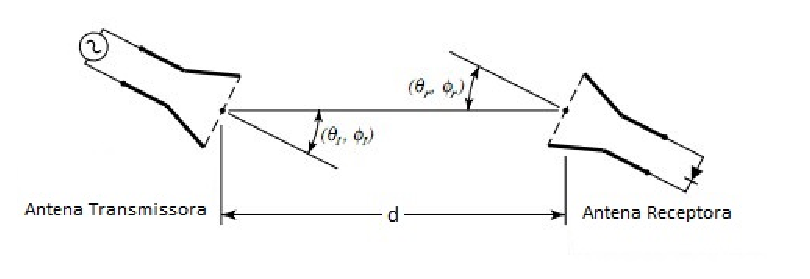
\includegraphics[keepaspectratio=true,scale=0.8]{figuras/antenas}
	\caption{Ilustração do posicionamento das antenas.}
	\label{antenas}
\end{figure}

O ganho $G(\theta,\phi)$ de uma antena é calculado de acordo com a equação \ref{dir1}.

\begin{equation}
\label{dir1}
    G(\theta,\phi) = eD(\theta,\phi)
\end{equation}

Sendo $e$ a eficiência da antena, que é o quanto da potência fornecida para seus terminais é irradiada, e $D(\theta,\phi)$ é a diretividade da antena, que é a razão entre a densidade de potência irradiada em uma direção específica e a densidade de potência irradiada nesta mesma direção caso ela fosse irradiada por uma antena isotrópica. Uma antena isotrópica é uma antena teórica que irradia a potência transmitida para todas as direções igualmente.

A equação \ref{com2} pode também ser calculada em dB como mostra a equação \ref{com3}.

\begin{equation}
\label{com3}
	10 \log_{10} P_{R} = 10 \log_{10} P_{R} + G_{T, dB} + G_{R, dB} - 20\log_{10}f - 20\log_{10}d+148
\end{equation}

$10 \log_{10} P_{R}$ e $10 \log_{10} P_{R}$ são dados em dBm (decibel milliwatt) pelo padrão de comparação ser o valor de $1mW$. $G_{T, dB}$ e $G_{R, dB}$ são dados em dBi (decibel isotrópico) devido ao padrão de comparação ser a densidade de potência irradiada por uma antena isotrópica. Os outros termos são dados em dB \cite{pauleletromagnetismo}.

Os valores dos parâmetros para o cálculo do link budget podem ser obtidos através do datasheet do transceptor \cite{ns:nrfl01}. A potência de saída é programada e tem disponível os valores de 0dBm, -6dBm, -12dBm e -18dBm para serem escolhidos, o valor utilizado no projeto é de 0dBm. Para saber qual a distância máxima é necessário saber a sensibilidade do receptor, pois é o valor mínimo de potência que deve ser recebida para que o sinal possa ser decodificado pelo módulo. A sensibilidade está relacionado a taxa de transferência de dados do sinal de acordo com a tabela  \ref{sensibilidade}.

\begin{table}[h]
\centering
\caption{Sensibilidade do RX \cite{ns:nrfl01}.}
\label{sensibilidade}
\begin{tabular}{|l|l|}
\hline
Taxa    & Sensibilidade \\ \hline
2Mbps   & -82dBm        \\ \hline
1Mbps   & -85dBm        \\ \hline
250kbps & -94dBm        \\ \hline
\end{tabular}
\end{table}

A taxa de transferência de dados utilizada no sistema foi de 1Mbps, consequentemente a sensibilidade do receptor é de -85dBm. O transceptor opera na frequência de 2.4. As antenas utilizadas no projeto são omnidirecionais com o ganho máximo de 2dBi, a direção de máxima irradiação da antena usada é ao seu redor, no plano onde também se encontra a outra antena a qual ela se comunica. Com estes valores especificados pode ser feita a estimativa da distância máxima entre as antenas, isolando a distância da equação \ref{com4}:

\begin{equation}
\label{com4}
	20 \log_{10} d = 2 + 2 - 187,6 + 148 + 85 = 49,4 \rightarrow d \approx 294,9 m
\end{equation}

O teste de distância foi feito afastando as antenas e verificando qual o máximo valor entre elas que era possível manter a conexão. Para medir esta distância foi usada a ferramenta “medir distância” do google maps utilizando como referência os pontos em que as duas antenas estavam localizadas quando perderam a conexão, como mostra a figura \ref{distancia_antena}.

\begin{figure}[h]
	\centering
	\includegraphics[keepaspectratio=true,scale=0.43]{figuras/distancia_antena}
	\caption{Distância máxima obtida para manter o link entre as antenas.}
	\label{distancia_antena}
\end{figure}

A distância máxima obtida foi de aproximadamente 300m. Tanto os valores teóricos como os experimentais mostram que as especificações dos equipamentos usados são suficientes para utilizá-los no projeto, pois a distância do tanque mais longe até a central é de 200m.

Os módulos de comunicação acoplados aos tanques e ao dispositivo central permitem a construção de uma rede para a troca de informações, a topologia de rede escolhida para esta aplicação foi a de rede em malha. A escolha pela topologia em malha foi feita pois ela permite conectar e desconectar tanques além de diminuir os problemas de alcance de dados, devido ao fato dos pacotes poderem passar por diversos dispositivos antes de chegarem a central.

Para a aplicação desta topologia de rede nRF24L01+ existe a biblioteca RF24Mesh projetada para o uso em Raspberry pi e nos microcontroladores ATmega. De acordo com o desenvolvedor da biblioteca, a mesma provê um sistema de endereçamento e roteamento automático dos módulos RF24 permitindo que grandes redes sem fio de sensores sejam construídas. Ela funciona utilizando um nó mestre, que no caso do projeto é a base, este nó mestre rastreia os IDs dos dispositivos que estão na rede, caso um dispositivo seja movido pela rede ela se auto organiza se reconfigurando novamente \cite{meshnetwork}.

O dispositivo dentro da rede pode estar em dois estados em relação à comunicação: escutando ou enviando informações. Ele passa a maior parte do tempo escutando a rede para verificar se chegou algum pacote para ele guardar ou reenviar pela rede, isto é feito através da função network.available() pertencente à biblioteca RF24Network a qual a biblioteca RF24Mesh utiliza em sua construção, quando um pacote é recebido um cabeçalho que vem juntamente com ele é lido para verificar qual o tipo de informação chegou (os tipos de informações trocadas serão apresentadas mais adiante). Este pacote de informação é lido então pela função network.read() onde são guardadas na memória para serem utilizadas posteriormente. Tanto a central quanto os tanques seguem este procedimento para receber as informações, ficam escutando a rede e caso alguma informação endereçada para eles cheguem eles verificam qual o cabeçalho do pacote que chegou, para saberem que tipo de pacote é aquele, e guardam a informação para seu uso posterior.

Quando está no horário de escrever algo (central escrever para algum nó específico ou algum nó escrever para a central) a função mesh.write() é então chamada, os parâmetros colocados dentro desta função são o pacote de informação a ser enviado, o cabeçalho que define o tipo de pacote que está sendo enviado e o nó para qual será enviado (caso seja a central este nó é o nó zero). É necessário também que a conexão seja verificada, para que, caso o dispositivo esteja enviando o pacote e não obtenha resposta, ele se reconfigure dentro da rede mudando seu endereço, estes dois processos são realizados pelas funções mesh.checkConnection() e mesh.renewAddress() respectivamente.

Os pacotes de informações enviados da central para os tanques são dois: um pacote contendo a hora local para que se possa programar o relógio interno sincronizando a rede, e o pacote contendo as informações acerca do horário de alimentação e quantidade de alimento. Já o pacote enviado dos tanques para a central contém informações acerca da bateria e dos sensores daquele tanque em específico. Estes pacotes são structs definidas no início do programa.

Pacote enviado do tanque para a central:

\begin{figure}[h]
\centering 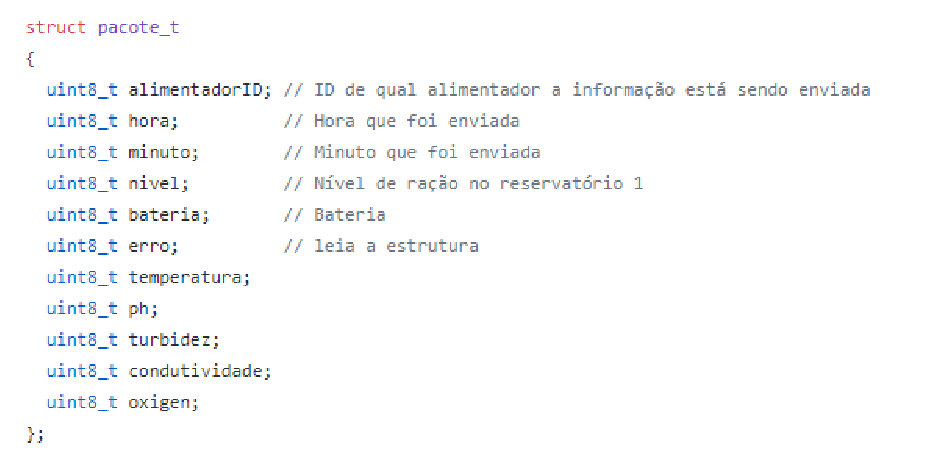
\includegraphics[keepaspectratio=true,scale=0.7]{figuras/pacote_t}
\label{pacote_t}
\end{figure}

\pagebreak

Pacote enviado da central para o tanque contendo informações acerca do horário de alimentação dos peixes:

\begin{figure}[h]
\centering 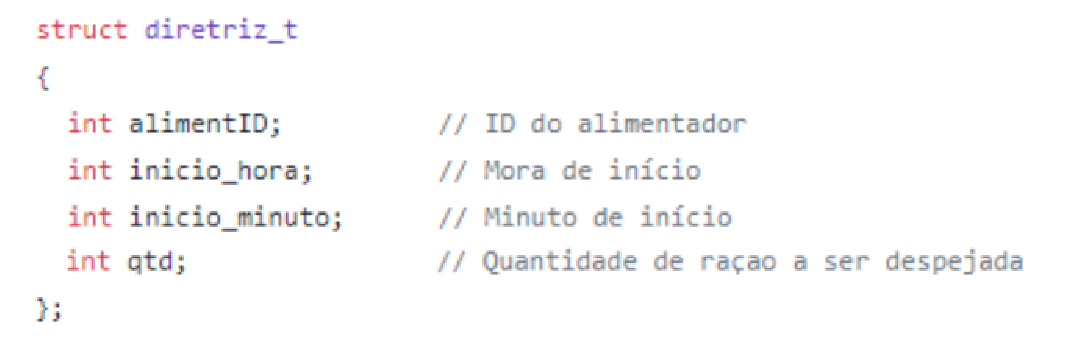
\includegraphics[keepaspectratio=true,scale=0.5]{figuras/diretriz_t}
\label{diretriz_t}
\end{figure}

\pagebreak

Pacote enviado da central para os tanques contendo as informações para a sincronização com o horário da base:

\begin{figure}[h]
\centering 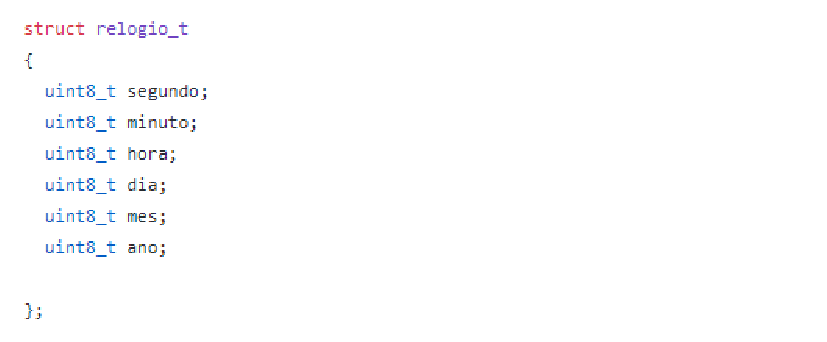
\includegraphics[keepaspectratio=true,scale=0.7]{figuras/relogio_t}
\label{relogio_t}
\end{figure}

\pagebreak

As informações enviadas para os tanques acerca da alimentação devem ser obtidas da aplicação web onde elas são colocadas, para isto um módulo python projetado pela equipe de software foi instalado na raspberry pi. Este módulo gera um arquivo .txt com estas informações que são lidas pelo programa projetado pela equipe de eletrônica e enviadas. As informações recebidas dos tanques pela central também são escritas em um arquivo .txt que é lido pelo módulo em python e enviado para o servidor web onde as informações serão exibidas ao usuário.


\subsection{Produção das Placas}

Método utilizado para a confecção da placa foi o fotográfico pois é o de melhor qualidade e riqueza de detalhes, este processo é constituído de 12 etapas:

1. Esquema elétrico e circuito eletrônico – Nessa etapa foi utilizado um software livre (Fritzing) para a criação do circuito tanto na protoboard quanto o circuito elétrico.


2. Layout do circuito impresso a partir do esquema elétrico -  O software Fritzing novamente foi utilizado gerando um fotolito que permitiu uma economia de matérias como percloreto de ferro e o tamanho das placas de fenolite.

3. Impressão do fotolito -  Foi utilizado uma impressora laser e um fotolito compatível com a impressora.

4. Sincronismo das faces - O alinhamento ocorreu apenas na camada existente

5. Limpeza da placa - A placa foi limpa com detergente e esponja vegetal

6. Aplicação do Dryfilm ou tinta fotossensível -  Neste caso foi utilizado a tinta foto sensível pois apesar de não ter uma qualidade tão elevada quanto o Dryfilm apresenta um custo menor

7. Alinhamento dos fotolitos e Fotografia - O alinhamento ocorreu apenas na camada existente

8. Revelação – Foi utilizada luz ultra violeta de 27w por 4 minutos a uma distância de 20 cm da placa

9. Corrosão – com percloreto de ferro

10. Remoção do dryfilm residual – A placa foi mergulhada em 250ml de uma solução de 10\% de hidróxido de sódio.

11. Furos para os componentes – A placa foi perfurada com uma broca de 1mm de diâmetro.

12. Aplicação do Verniz para proteção contra corrosão.

A figura \ref{placa} apresenta o projeto feito em software da placa principal

\begin{figure}[h]
\centering \includegraphics[keepaspectratio=true,scale=0.7]{figuras/placa}
\caption{Projeto da PCB.}
\label{placa}
\end{figure}


A figura \ref{placapronta} mostra a placa final produzida para o projeto.

\begin{figure}[h]
\centering \includegraphics[keepaspectratio=true,scale=0.3]{figuras/placa_pronta}
\caption{Placa pronta.}
\label{placapronta}
\end{figure}
